\section{Literature Review} 
\label{section:liteReview}

The literature review is structured as in Figure \ref{fig:org_lit_review}. In Section \ref{aircraft_maint_practice}, we describe the general practice in aircraft maintenance and introduce relevant terminologies. Depending on the planning horizon length, there are two types of aircraft maintenance planning problems, namely short-term planning problems reviewed in Section \ref{aircraft_maint_practice} and long-term planning problems reviewed in Section \ref{aircraft_maint_practice}. As this paper is concerned with a large-scale joint optimization problem, we further review popular solution algorithms used to solve large-scale optimization problems, particularly the decomposition-based solution approaches with applications in aviation in Section \ref{sec:SolApproach}. Finally, major research gaps are summarized in Section \ref{sec:LitRevSummary}.


\begin{figure}[htbp]
    \centering
    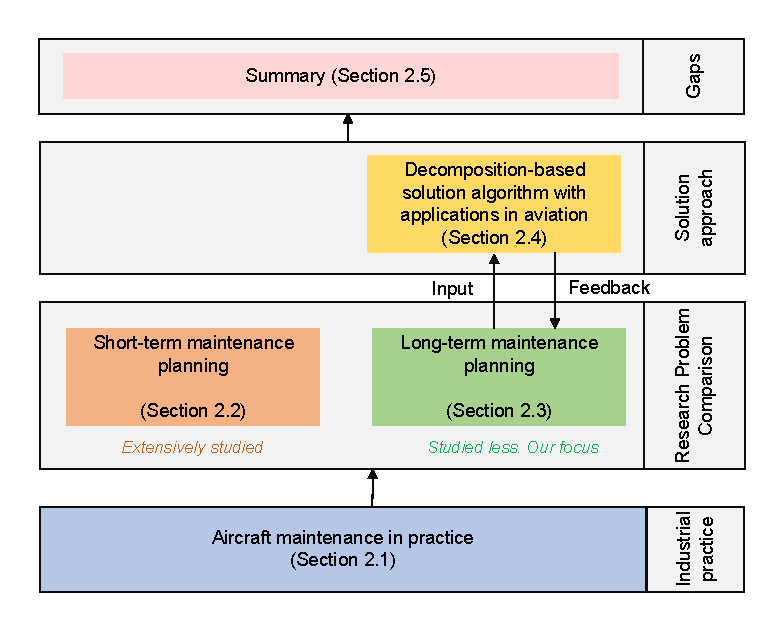
\includegraphics[width=0.65\linewidth]{literature_framework.pdf}
    \caption{Organization of the literature review}
    \label{fig:org_lit_review}
\end{figure}



\subsection{Aircraft maintenance in practice }
\label{aircraft_maint_practice}
In civil aviation, aircraft undergo various maintenance activities at predetermined intervals. These maintenance activities are generally classified as preventive (scheduled) or corrective (unscheduled). 
Preventive maintenance is a proactive process performed to prevent system failures \citep{van2013aircraft,tseremoglou2024condition}. This type of maintenance is organized into four key types of checks, commonly referred to as lettered checks: A, B, C, and D checks \citep{preventive_vs_on-condition}. The intervals for these checks are tracked using several indicators, including calendar days, flight cycles, and flight hours. These intervals are well defined in the maintenance program \citep{icao2019aircraft}. For instance, an A check is typically conducted every 600–2,000 flight hours, 200–300 flight cycles, or 60–150 calendar days. Many airlines have discontinued B checks to reduce the overlap with A checks \citep{lagos2020dynamic}. A new C check is due after approximately 16,000 flight hours, 2,000 flight cycles, or 24–26 months, while D checks, which are the most extensive, take place roughly every 6–10 years \citep{naatypesofaviationmaint}. Although in some studies, those checks are named A-check, B-check, and so on, we do not keep the hyphen between the letter and ``check'' to be consistent with the practice of the collaborating airline. \color{black} Depending on its fleet characteristics (such as mix and age), an airline usually creates its own maintenance program to address its specific needs. In contrast with preventative maintenance, corrective maintenance involves unscheduled tasks that are necessary to restore an aircraft system to optimal condition after a failure has occurred \citep{eddarhri2022towards}.

Depending on the maintenance location, aircraft maintenance can also be classified as line vs base (hangar) maintenance. Line maintenance refers to tasks carried out at the gate or on the apron.  Line maintenance activities usually occur during an aircraft's ground time window or are called ``maintenance opportunity'' \citep{villafranca2025aircraft}. \color{black}  Any maintenance work that cannot be completed in the above areas is classified as base or hangar maintenance \citep{van2013aircraft}. The execution of these maintenance tasks largely depends on an airline's capabilities. Some airlines carry out maintenance in-house at their own facilities, often located in airport hangars, while others choose to outsource the work to third-party MRO providers.


\subsection{Short-term maintenance planning for aircraft}
\label{subsect:maint_routin_problm}
To better understand the maintenance planning problem, we briefly discuss the airline scheduling process and then focus on the short-term problem variants, particularly the well-studied aircraft maintenance routing problem (AMRP) and the line maintenance scheduling problem (LMSP). 
\color{black}


There are four types of scheduling problems in airline operations, namely flight scheduling, fleet assignment, aircraft maintenance routing, and crew scheduling, which are solved sequentially \citep{barnhart2004airline}.
As illustrated in Figure~\ref{fig:airline_scheduling problem}, the airline scheduling process begins with flight scheduling, at least a few months in advance. In this stage, an airline identifies the markets to serve, the frequency of flights, and the timing of these flights. Once flight schedules are established, specific aircraft types are assigned to flight legs of the identified schedules during the fleet assignment process \citep{clarke1997aircraft}. Many factors, such as aircraft capacity, range, and fuel efficiency, are considered during fleet assignment to match the most suitable aircraft type with each flight leg \citep{gopalan1998aircraft}. Following fleet assignment, aircraft maintenance routing deals with the assignment of each individual aircraft to flight legs. A rotation is a series of flight legs with the destination of a leg as the origin of the immediate next leg, while the final destination is the same as the initial origin of an aircraft, thus completing a tour. While completing the rotation, an aircraft is mandated to visit certain maintenance facilities according to maintenance regulations. Additionally, in crew scheduling, airlines assign crew members (flight attendants and pilots) to flight legs. 


\begin{figure}[htbp]
    \centering
    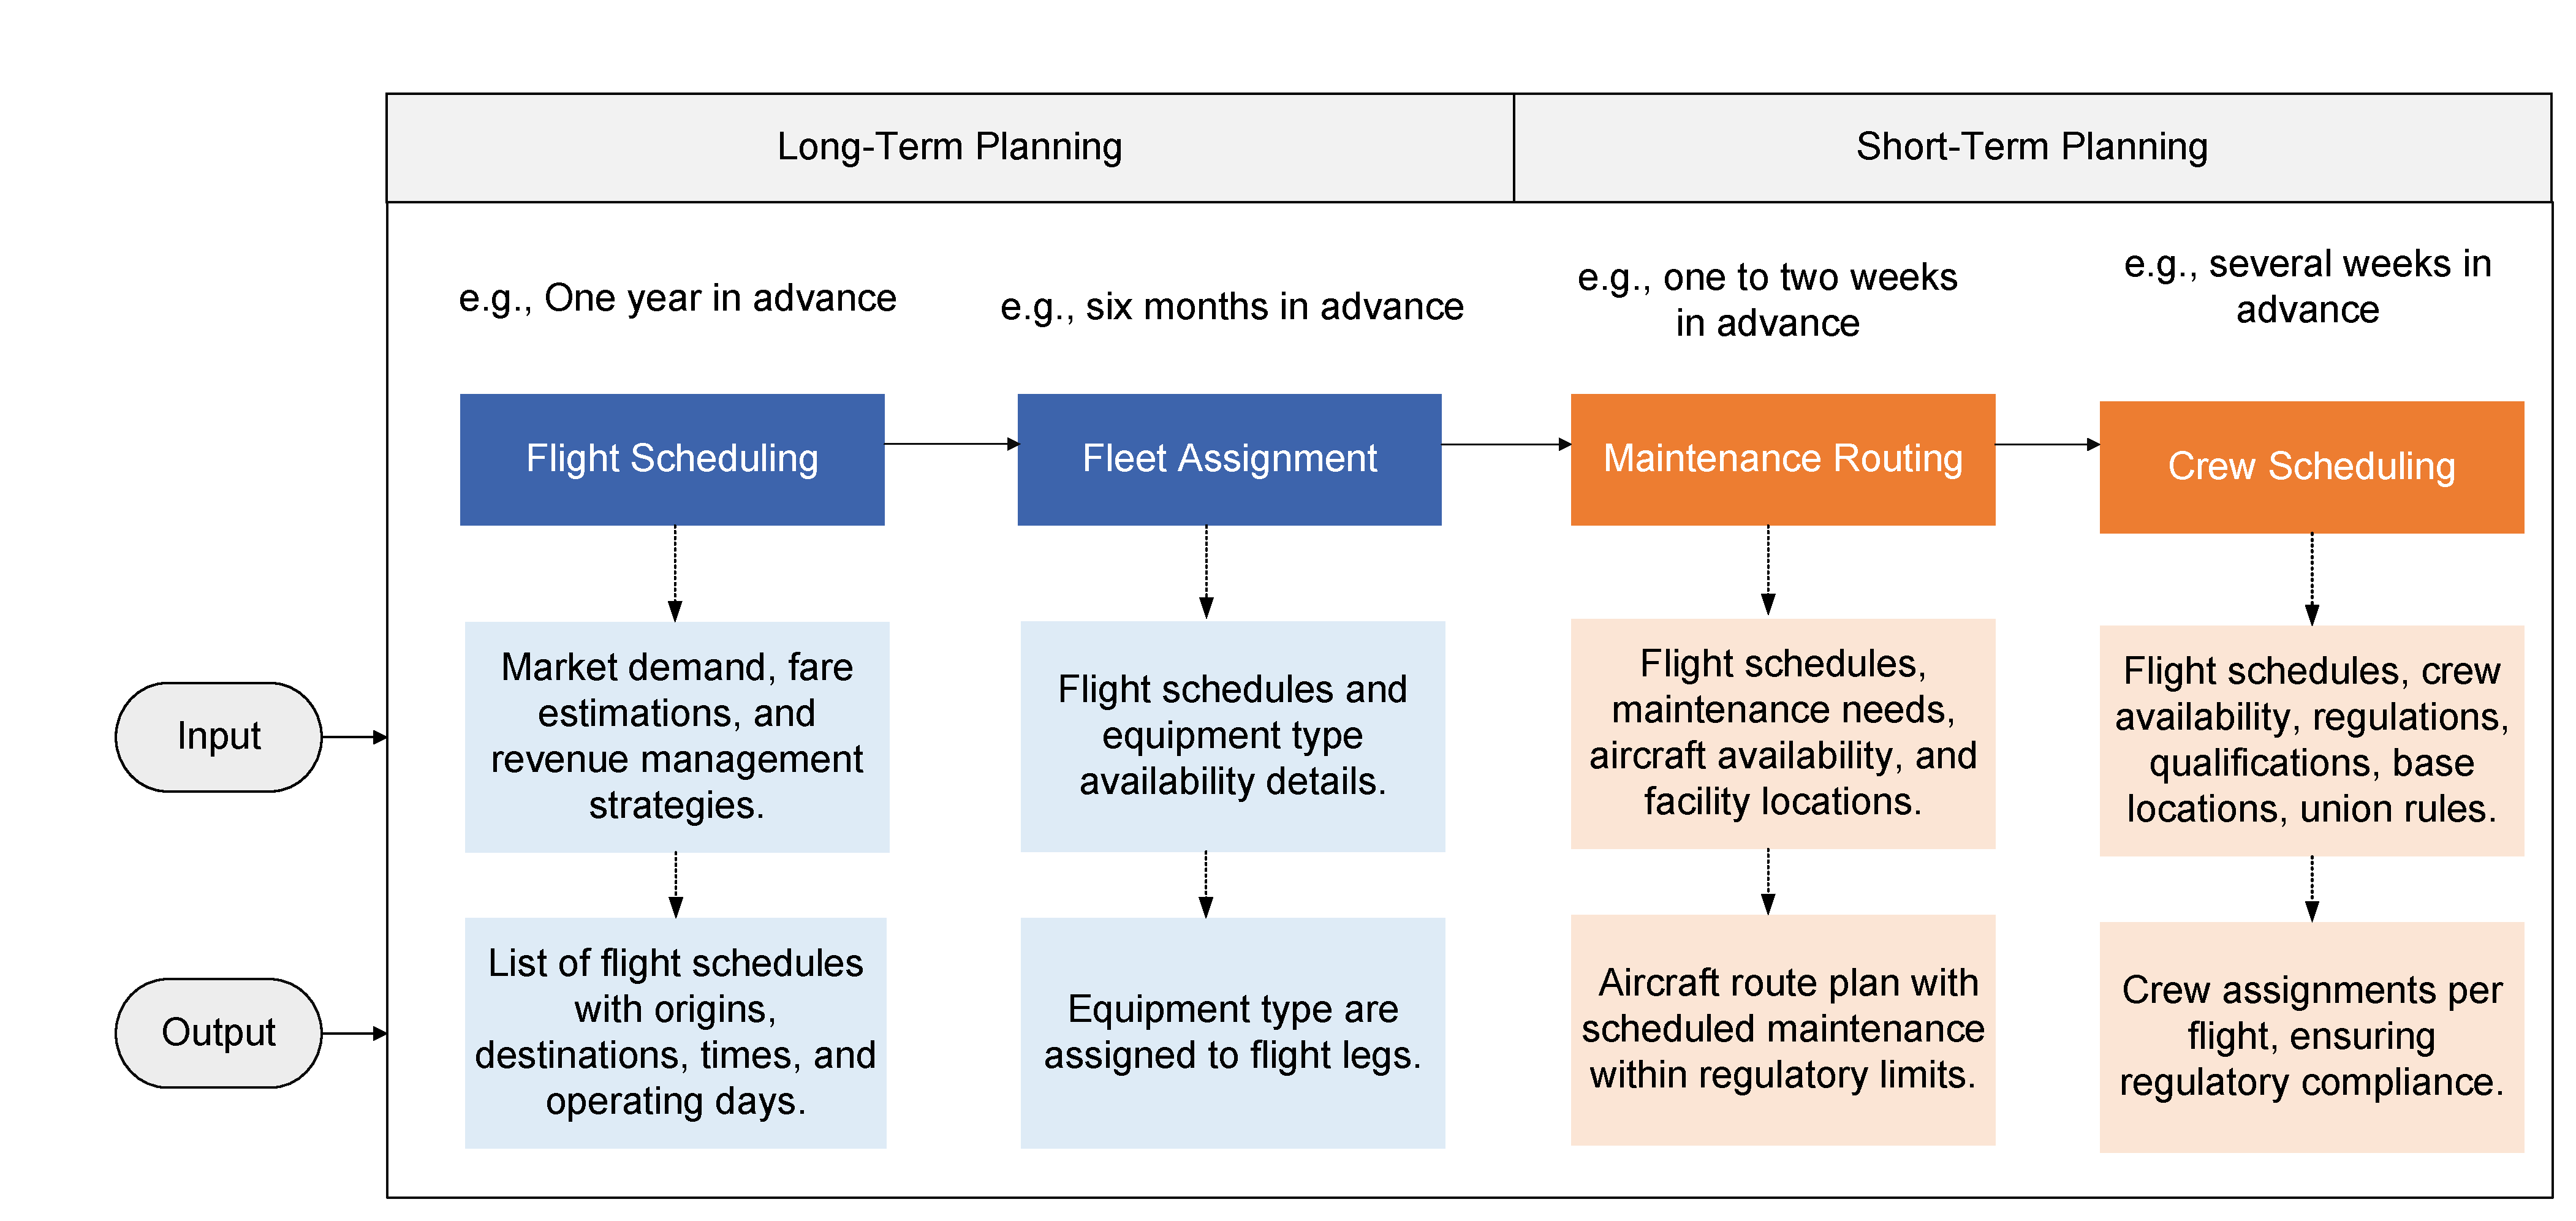
\includegraphics[width=\linewidth]{airlineschedulingv7.pdf}
    \caption{Overview of an airline scheduling process}
\label{fig:airline_scheduling problem}
\end{figure}

Although all the above four optimization problems have been widely studied in the literature, we next focus on the AMRP, considering the relevance of the AMRP to our research. 
Given \color{black} a set of aircraft and corresponding flight schedules, the AMRP is concerned with assigning aircraft to sequences of flights (referred to as ``routes'') while ensuring both operational and maintenance requirements are met. This means that a suitable aircraft must cover every flight leg, and necessary maintenance must be performed without disrupting scheduled operations. Typically, the planning horizon for AMRP usually spans two to four days \citep{feo1989flight, eltoukhy2017airline}, though in some cases, it may extend up to a week \citep{sriram2003optimization, he2023maximizing}. 
We further briefly comment on the size of AMRP instances. For example, \cite{ruan2021reinforcement} considered nine real-world instances from Egyptair. The number of flight legs varies from 40 to 400; the fleet size varied from 8 to 42; the number of maintenance stations involved ranged from 4 to 9. 



In addition to the AMRP, we further review other short-term aircraft maintenance planning problems without involving aircraft routing. In an LMSP study, \cite{villafranca2025aircraft} focused on deciding what maintenance tasks should be outsourced versus performed in-house and determining the start times for these in-house tasks.
The study specifically examined line maintenance operations carried out during maintenance opportunities, with a planning horizon of 24 hours.



\subsection{Long-term maintenance planning for aircraft}
\label{sec:long_termPlanningRev}

While the planning horizon in short-term maintenance planning problems is typically no more than several weeks, the long-term aircraft maintenance planning problem is defined over a much longer time horizon, spanning several months or even years \citep{ma2022tackling}. The differing planning horizon length implies a few other key differences. First, in the AMRP, detailed flight departure and arrival times are known and a series of flight legs are built into an aircraft route; by contrast, detailed flight schedules are unavailable for an extended planning horizon, such as six months, no aircraft routing decisions are involved in a long-term aircraft maintenance planning study. 
Second, due to AMRP's short-term nature, it primarily considers routine checks that occur quite frequently, e.g., once every a few days \citep{sriram2003optimization}. By contrast, the long-term aircraft maintenance planning usually involves major checks, such as the C checks that are needed infrequently (e.g., once every a few months).

Given the above differences, we present an in-depth review of only those studies focusing on long-term planning problems.


\cite{boere1977air} documented innovative efforts made by Air Canada in the 1970s to replace a manual procedure for long-term aircraft maintenance scheduling with the Aircraft Maintenance Operations Simulation (AMOS) model. AMOS was essentially a simulation system where a priority-based scheduling heuristic was incorporated, because \cite{boere1977air} argued that other modeling or solution approaches, including mixed integer programming, dynamic programming, and out-of-kilter algorithms, were unsuitable. Their optimization objective was to minimize the lost aircraft flying hours and it was concluded that a 5\% maintenance cost and labor reduction was achieved. A related study \cite{deng2020practical} followed six major conditions for maintenance scheduling, originally introduced in \cite{boere1977air}, and made two more assumptions. They sought to determine whether a check for an aircraft should start on a given day over a long planning horizon (such as four years), following a dynamic programming (DP) framework. They tested their solution method in a case study based in Europe, which involved a fleet of 45 A320 aircraft. A single maintenance base was considered, as they focused on scheduling decisions only. The DP approach might face computer memory issues for large instances. 


% However, several extensions to \cite{deng2020practical} work were made, and we discussed them as follows.  
We next review a few studies built upon \cite{deng2020practical}. \cite{andrade2021aircraft} 
utilized a Deep Q-learning algorithm to optimize long-term maintenance scheduling policies developed by  \cite{deng2020practical}. Their methodology prioritized the schedule of C checks over A checks, given that C checks require more ground time and significantly influenced the scheduling of subsequent A checks. 
Rather than minimizing maintenance costs, they focused on maximizing flight utilization between two consecutive checks to increase aircraft availability in the long term. The test instances involved in this analysis were the same as those of \cite{deng2020practical}.
Their experimental results demonstrated that reinforcement learning produced a more efficient maintenance plan than dynamic programming adopted by \cite{deng2020practical}.
\color{black}
\cite{van2022robust} developed an integer programming model to generate a long-term heavy maintenance schedule for checks, which comprises the C and the D checks. Given a sequence of C checks, the D is merged with the C check, which is carried out after every two C cheeks have been scheduled. Their main decision was to determine the start of a maintenance check for a particular aircraft. Given the increase in complexity, they solved the optimization problem using a genetic algorithm (GA) that was validated on synthetic aircraft maintenance data. \cite{van2022robust}  ran the DP solution approach developed by  \cite{deng2020practical}, and then compared the results of GA with that of DP. In terms of the practicality of the model, they considered some applicable constraints such as utilization, maintenance, and operational constraints. However, they did not consider explicitly some practical capacity constraints at the maintenance stations, such as the man hours available at the station. A single maintenance station was considered. 

Rather than merely focusing on check scheduling only,  \cite{deng2020practical} further incorporated task allocation and shift planning into a decision support system (DSS). \color{black} The DSS took input from multiple sources, such as the maintenance planning document, fleet status, operational constraints, task workload, and workforce availability. It employed a top-down optimization approach in which, at the task allocation level, it focused on allocating tasks to a maintenance opportunity. 
% A maintenance opportunity, as defined by \cite{deng2021novel}, is a given time window for performing a specific check with corresponding capacity. 
However, the DSS did not consider aircraft-to-station assignment as it considered only a single maintenance station. In addition, the DSS only considered the general man-hour capacity constraints available at their maintenance hangar. However, given the supposed practicality of this framework, other necessary real-world capacity constraints, such as the number of checks a station can handle (line count limit) and the possibility of handling two C checks per day or combining both A and C checks and so on, remain vital. 

Other long-term maintenance planning studies are also reviewed. Focusing on maintenance schedules for Taiwan's major airline operator and its client's fleet,
\cite{yan2008long} presented an integer programming model for the long-term aircraft maintenance planning considering a single airport, with multiple hangars, and a heterogeneous fleet. Their core decision was when an aircraft should be assigned for maintenance at which hangar. Over their planning horizon, each aircraft needed at most one check. Therefore, they explicitly defined a single maintenance due date for an aircraft. They did not specify where A and/C checks were conducted in their study. If A checks were involved, there should be multiple A checks over a one-year period, while their model was unable to address that. Their optimization model was solved directly by a commercial solver (CPLEX) after two objectives were merged into one with a weighting method. As their case study involved 68 aircraft and one airport, they did not design any custom solution algorithms to address larger problem instances. 


We present the summary of these studies for long-term aircraft maintenance planning problem in Table~\ref{tab:sum_aircraft_maint}. We further comment that many practical constraints, such as aircraft rotation requirement, A check limit, C Check limit, and station access limit, are absent in those existing long-term studies. In addition, the preference of an aircraft to be maintained at a particular station, which is preferred by major airlines, has not been considered in those existing studies.  It should be noted that all those studies in Table~\ref{tab:sum_aircraft_maint} considered a single maintenance station, although a major airline will likely use multiple maintenance stations when its fleet is sufficient large.


\begin{table}[htbp]
\centering
\caption{Summary of long-term aircraft maintenance planning studies}
\label{tab:sum_aircraft_maint}
\resizebox{\textwidth}{!}{%
% \fontsize{14}{20}\selectfont
\begin{tabular}{lccccccl}
\hline
\multirow{3}{*}{Study} & \multirow{3}{*}{Data type} & \multirow{3}{*}{\begin{tabular}[c]{@{}c@{}}Maintenance \\ check type\end{tabular}} & \multirow{3}{*}{\begin{tabular}[c]{@{}c@{}}Number of \\ maintenance \\ check types\end{tabular}} & \multirow{3}{*}{\# of stations} & \multirow{3}{*}{\begin{tabular}[c]{@{}c@{}}Aircraft \\ fleet size\end{tabular}} & \multirow{3}{*}{Fleet type} & \multirow{3}{*}{Solution approach} \\
 &  &  &  &  &  &  &  \\
 &  &  &  &  &  &  &  \\ \hline
\cite{boere1977air} & R & A,B,C & 3 & 1 & - & HT &  Simulation-based heuristic \\
\cite{yan2008long} & R & - & - & 1 & 68 & HT &  Exact Algorithm \\
\cite{deng2020practical} & R & A,C & 2 & 1 & 45 & HM & Dynamic Programming \\
\cite{deng2021novel} & R & A,C & 2 & 1 & 66 & HM &  Worst-Fit Decreasing Algorithm \\
\cite{andrade2021aircraft} & R & A,C & 2 & 1 & 45 & HM & Deep Q-learning \\
\cite{van2022robust} & S & C,D & 2 & 1 & 40 & - &  Genetic Algorithm \\
\textbf{Our work} & \textbf{R} & \textbf{A,C01-C10} & \textbf{11} & \textbf{15} & \textbf{$>$800} & \textbf{HT} &  \textbf{Decomposition-based  Approaches} \\ \hline
\end{tabular}%
}
\begin{minipage}{\textwidth} 
    \footnotesize
    \vspace{1mm}
    R - Real-world data;$\quad$ S - Simulated data; $\quad$
     HT - Heterogeneous Fleet;$\quad$
     HM - Homogeneous Fleet
 \end{minipage}
\end{table}


As shown in Table~\ref{tab:sum_aircraft_maint}, existing studies addressing long-term aircraft maintenance planning problems have all been conducted on a small to medium-sized scale. This is evident from the limited number of aircraft (fewer than 70), and the number of maintenance stations (limited to only one).
% , and the parameters defining maintenance capacity.
Given that solving these problems using exact methods with commercial solvers has become impractical even for these small-scale problems as a result of complexities, fast heuristics are usually developed to tackle these problems \citep{wang2024collaboration}.

We note that some seemingly relevant studies are not reviewed in detail, as they focus on a more granular level. For example, \cite{chen2024resource} broke down a single C check of an aircraft into hundreds of maintenance tasks and aimed to optimize the task scheduling to minimize the makespan (i.e., the duration of the C check). Given the focus of \cite{chen2024resource} on a single check, it is not directly relevant to the core research problem of this paper. 


\subsection{Decomposition-based solution algorithm with applications in aviation}
\label{sec:SolApproach}
% As shown in Table~\ref{tab:sum_aircraft_maint}, previous studies addressing long-term aircraft maintenance planning problems have all been conducted on a small to medium-sized scale. This is evident from the limited number of aircraft (fewer than 70), the number of maintenance stations (limited to only one), and the parameters defining maintenance capacity. Given that solving these problems using exact methods with commercial solvers has become impractical for these small scale problems, some studies have developed heuristic solution approaches, 
% to tackled these problems. However, they remain impractical when the problem size grows. For instance, \cite{deng2020practical} observed that although dynamic programming can yield exact solutions, it suffers from the curse of dimensionality, rendering it impractical for large-scale instances due to excessive computational requirements.


As no studies have tackled the joint optimization of aircraft maintenance scheduling and station assignment decisions in the literature, no applicable solution algorithms are available. To motivate the solution algorithm design for the long-term aircraft maintenance optimization problem under consideration in this paper, we briefly review several common decomposition-based solution strategies for solving large-scale optimization problems in aviation. 
For instance, \cite{sama2013rolling} utilized the rolling horizon decomposition approach to determine aircraft scheduling while considering busy traffic situations resulting from a large number of delayed aircraft. They achieved this by updating the scheduling decision based on new traffic information. 
In contrast, \cite{diao2018sequence} adopted a different decomposition solution approach by using a hybrid decomposition method that combines Dantzig-Wolfe decomposition and column generation for air traffic management. Similarly, \cite{wang2025airport} developed a customized decomposition approach that hierarchically separates strategic flight scheduling from operational adjustments to solve the airport slot allocation problem. 



\color{black}
\subsection{Summary}
\label{sec:LitRevSummary}
Although the literature on aircraft maintenance optimization is extensive, the vast majority of the current literature is devoted to the short-term planning problem, which is different from the long-term aircraft maintenance planning problem in terms of the planning horizon length and type of decisions involved. An in-depth review of the handful long-term aircraft maintenance planning studies produces the following research gaps:
\begin{enumerate}
    \item The existing long-term aircraft maintenance planning studies have focused primarily on the timing of maintenance checks and have not incorporated aircraft-to-station assignments.
    For major airlines with a large set of spatially distributed maintenance facilities, aircraft-to-station assignment decisions (where to conduct maintenance) are as necessary as the scheduling decision (when to conduct maintenance). 
    % For a major airline operating a large fleet and a network of maintenance facilities, the joint optimization of two interrelated decisions, namely scheduling (when to conduct maintenance) and assignment (where to conduct maintenance) is essential. 
    At present, none of the existing studies have attempted to optimize them jointly and address the above practical need,  possibly because jointly optimizing them is quite challenging.
    \item Although some maintenance-related constraints, such as man-hour limits, are considered in the existing aircraft maintenance planning studies, many practical constraints remain unaddressed. For example, each maintenance station is constrained by the number of aircraft it can accommodate, referred to as the line count. The number of C checks that can be performed on an aircraft is 0, 1, or 2, while C checks from different groups cannot be carried out simultaneously.
    The aircraft rotation constraint is also missing in the existing aircraft maintenance planning studies. Those constraints should be considered to improve the realism of aircraft maintenance planning. 
    \item The current studies on the long-term aircraft maintenance planning problem have primarily focused on small to medium-sized problems. For instance, the maximum fleet size is less than 100 in the current literature while a major airline may operate hundreds of aircraft in the real world. As a result, the solution approaches developed for these problems might be inadequate for large, realistic problem instances.
\end{enumerate}

To address the identified research gaps, a practical integrated optimization method for aircraft maintenance scheduling and assignment at a large scale is essential, which is presented in this study.  